 \section{Introduction}


\begin{frame}{Introduction}
       \tableofcontents[sectionstyle=show/hide, hideothersubsections]
    \begin{center}
    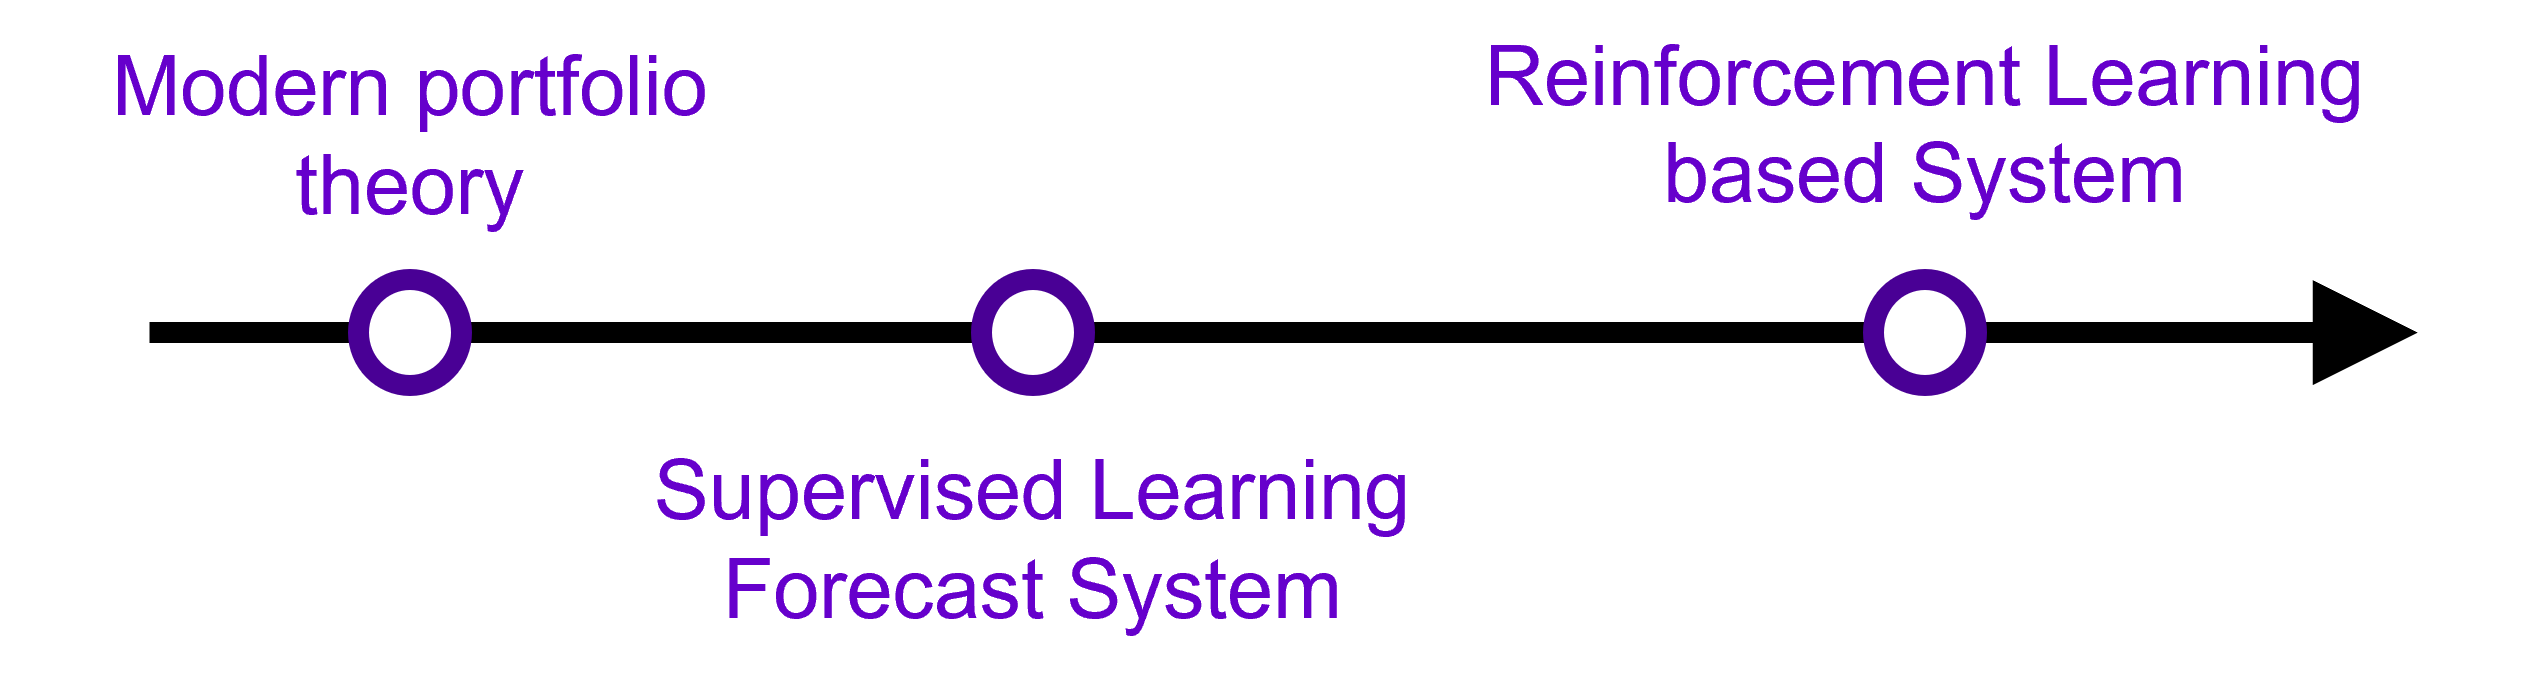
\includegraphics[width=10cm]{images/portfolio_introduction.png}
    \end{center}
\end{frame}


\subsection{Objective}
\begin{frame}
\frametitle{Objective}
\begin{columns}
\begin{column}{0.55\textwidth}
Incorporate DRL-based System with investor preference(\alert{risk preference}).


\begin{block}{Objective}
\begin{enumerate}
    \item Produce portfolios with different risks by adjusting parameters..
    \item Outperform constant rebalanced portfolio (CRP)
\end{enumerate}
\end{block}
\end{column}
\begin{column}{0.45\textwidth}
\begin{center}
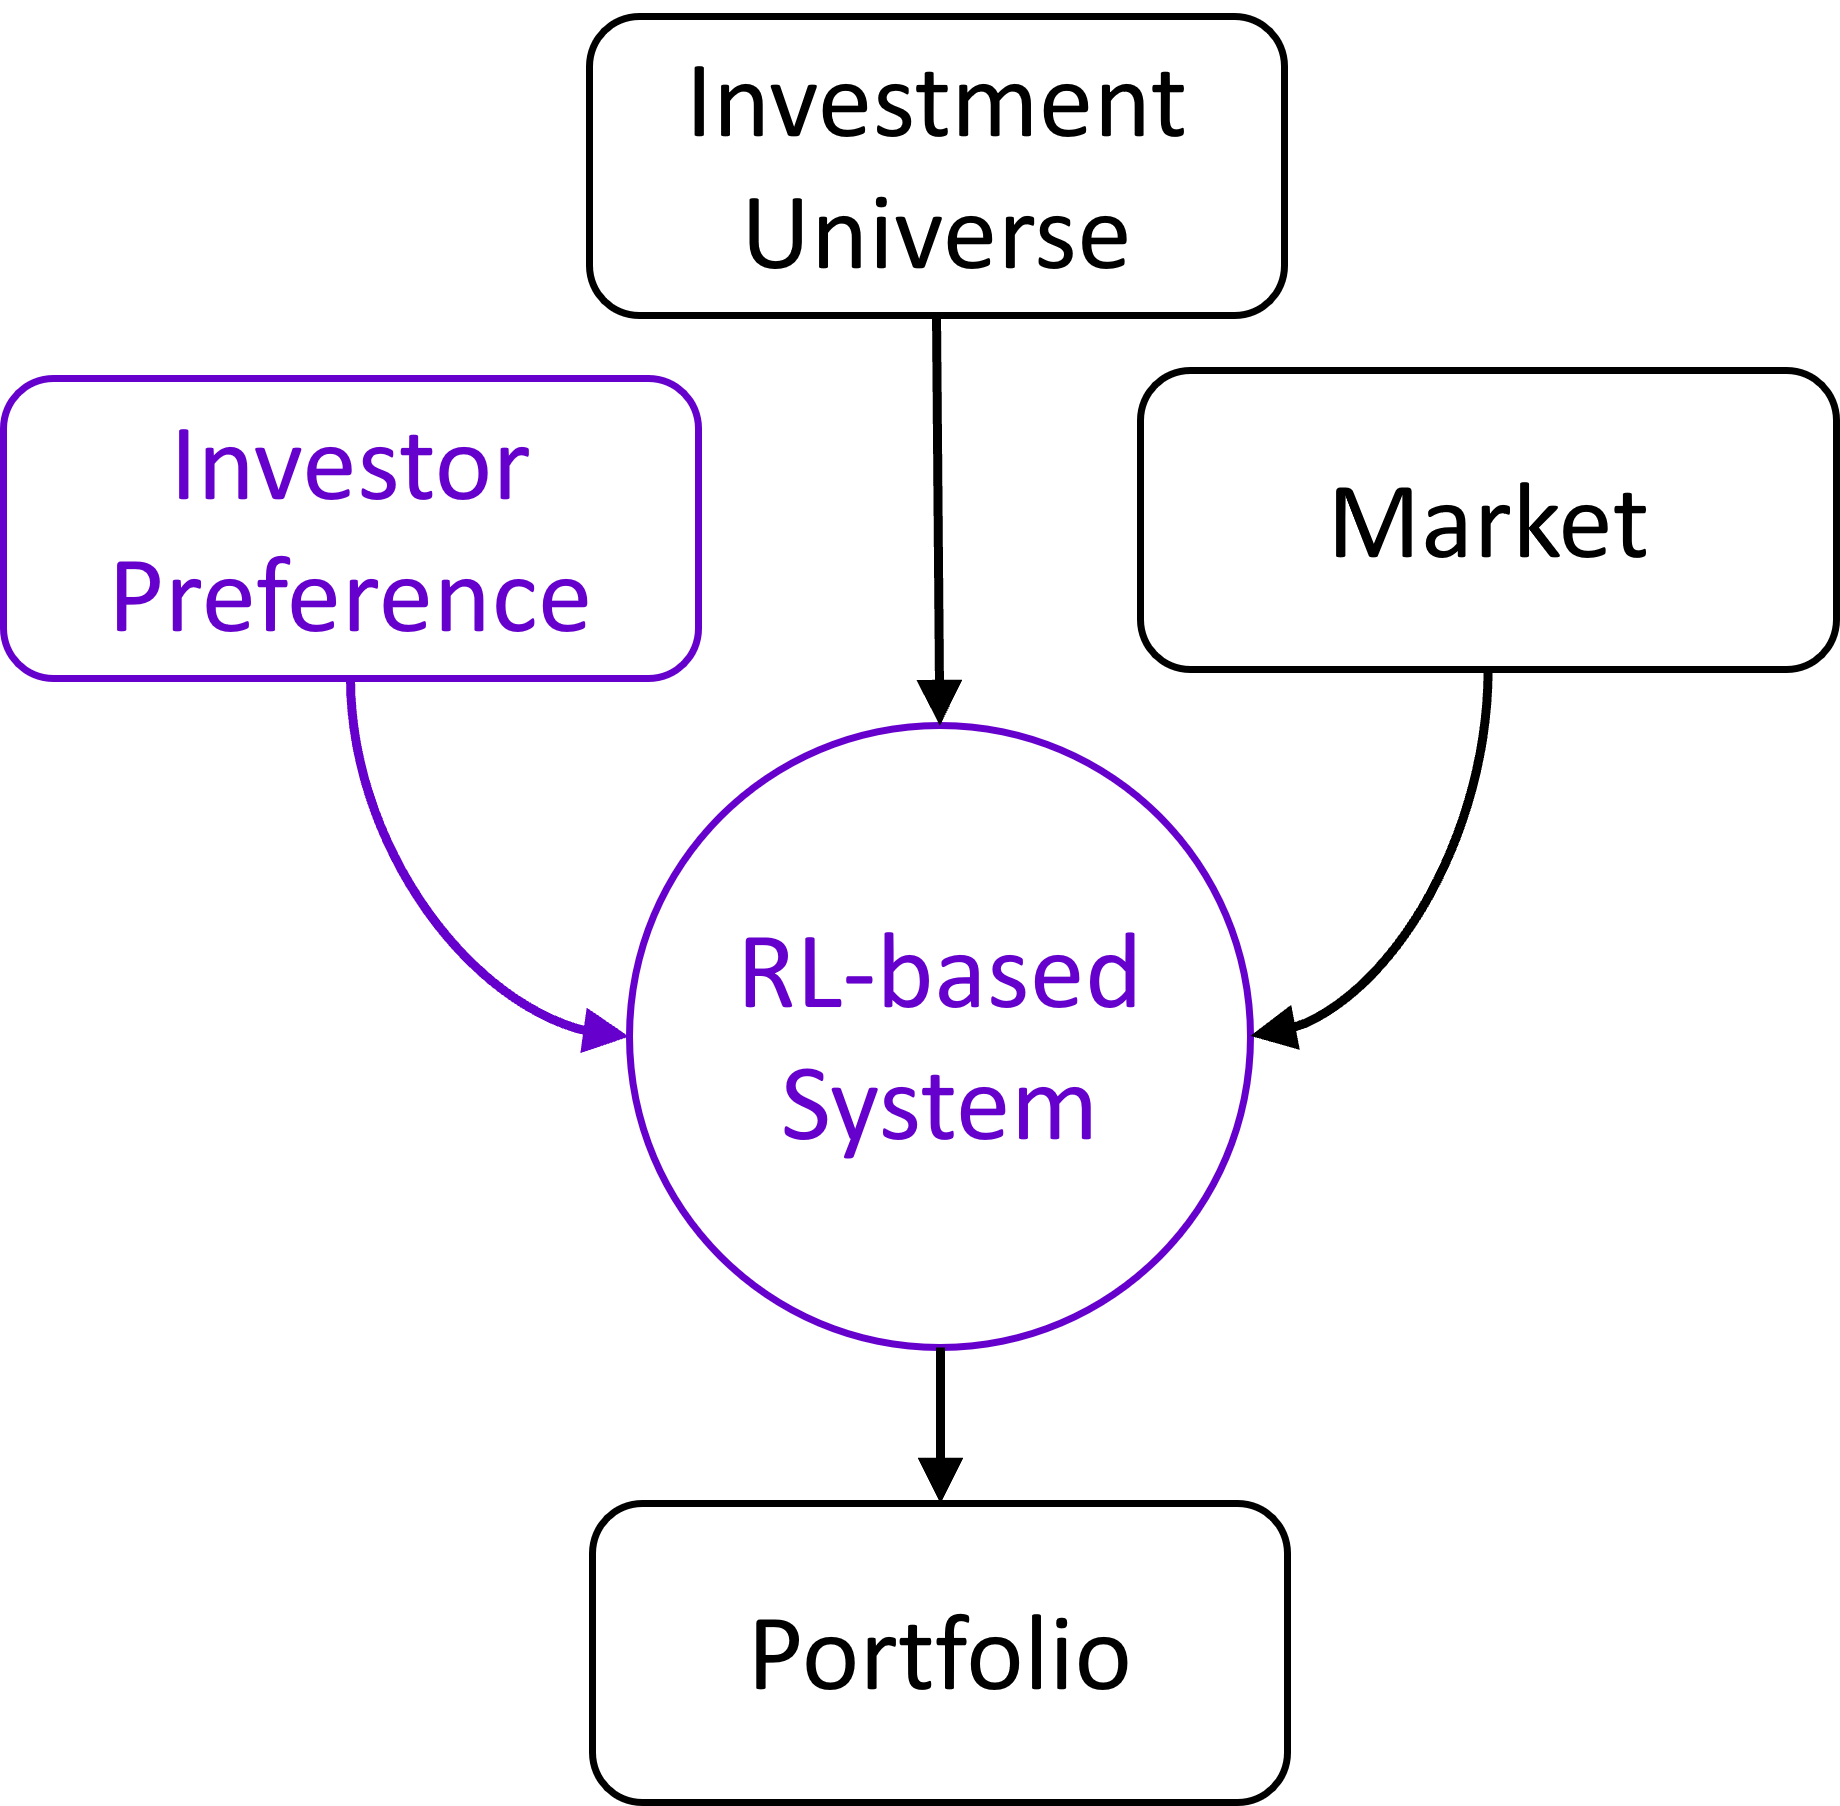
\includegraphics[width=4.8cm]{images/rl2.png}
\end{center}
\end{column}
\end{columns}
\end{frame}


\begin{frame}
\frametitle{Portfolio Management System}
\begin{columns}
\begin{column}{0.55\textwidth}
\begin{block}{Portfolio}
Collection of financial investments
\end{block}
\begin{block}{Portfolio Management System}
A system produces portfolios based on investment universe, the market, and investor preference
\end{block}
\begin{block}{Terms}
    Wealth: Total value of the portfolio
    Profit: Wealth gain between each trade
\end{block}
\end{column}

\begin{column}{0.45\textwidth}
\begin{center}
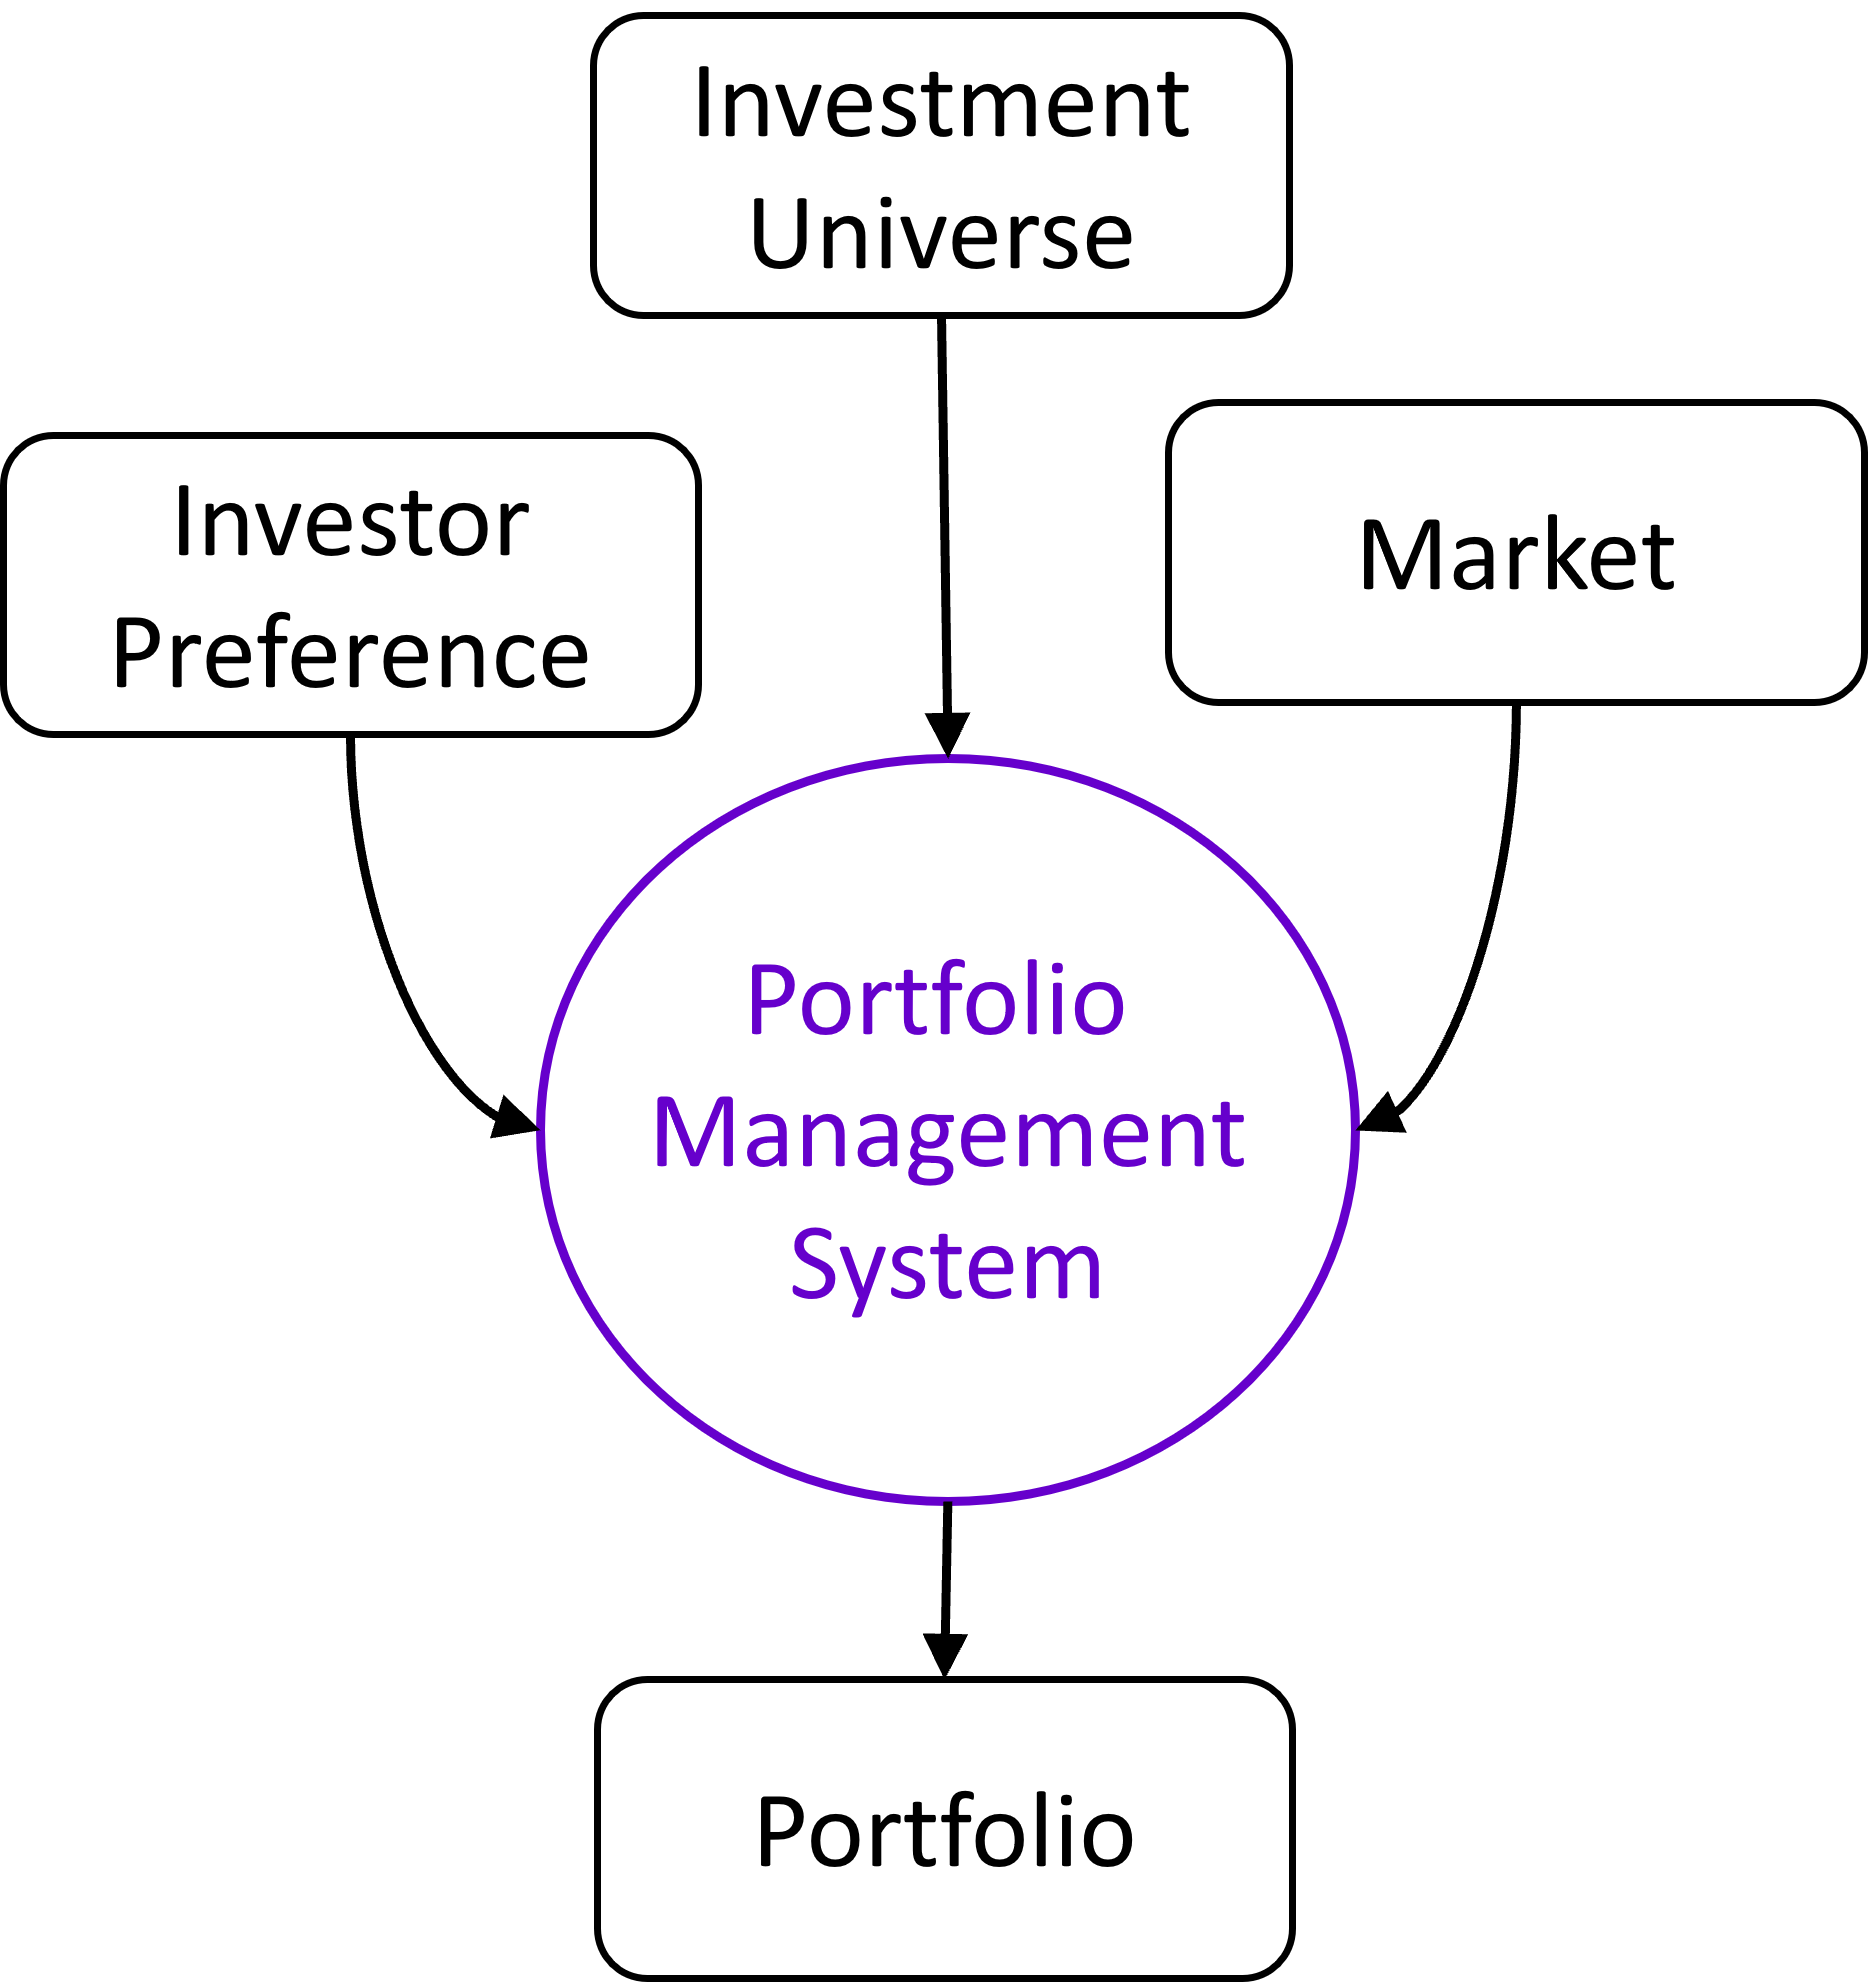
\includegraphics[width=4.8cm]{images/portfolio_management_system.png}
\end{center}
\end{column}
\end{columns}
\end{frame}


\subsection{Modern Portfolio Theory}
\begin{frame}
\frametitle{Modern Portfolio Theory (MPT)}
\begin{columns}
\begin{column}{0.55\textwidth}
MPT produces portfolios with maximum expected return from given risk (variance) or vice versa base on the forecasts of future performance (expected return and variance)
\begin{center}
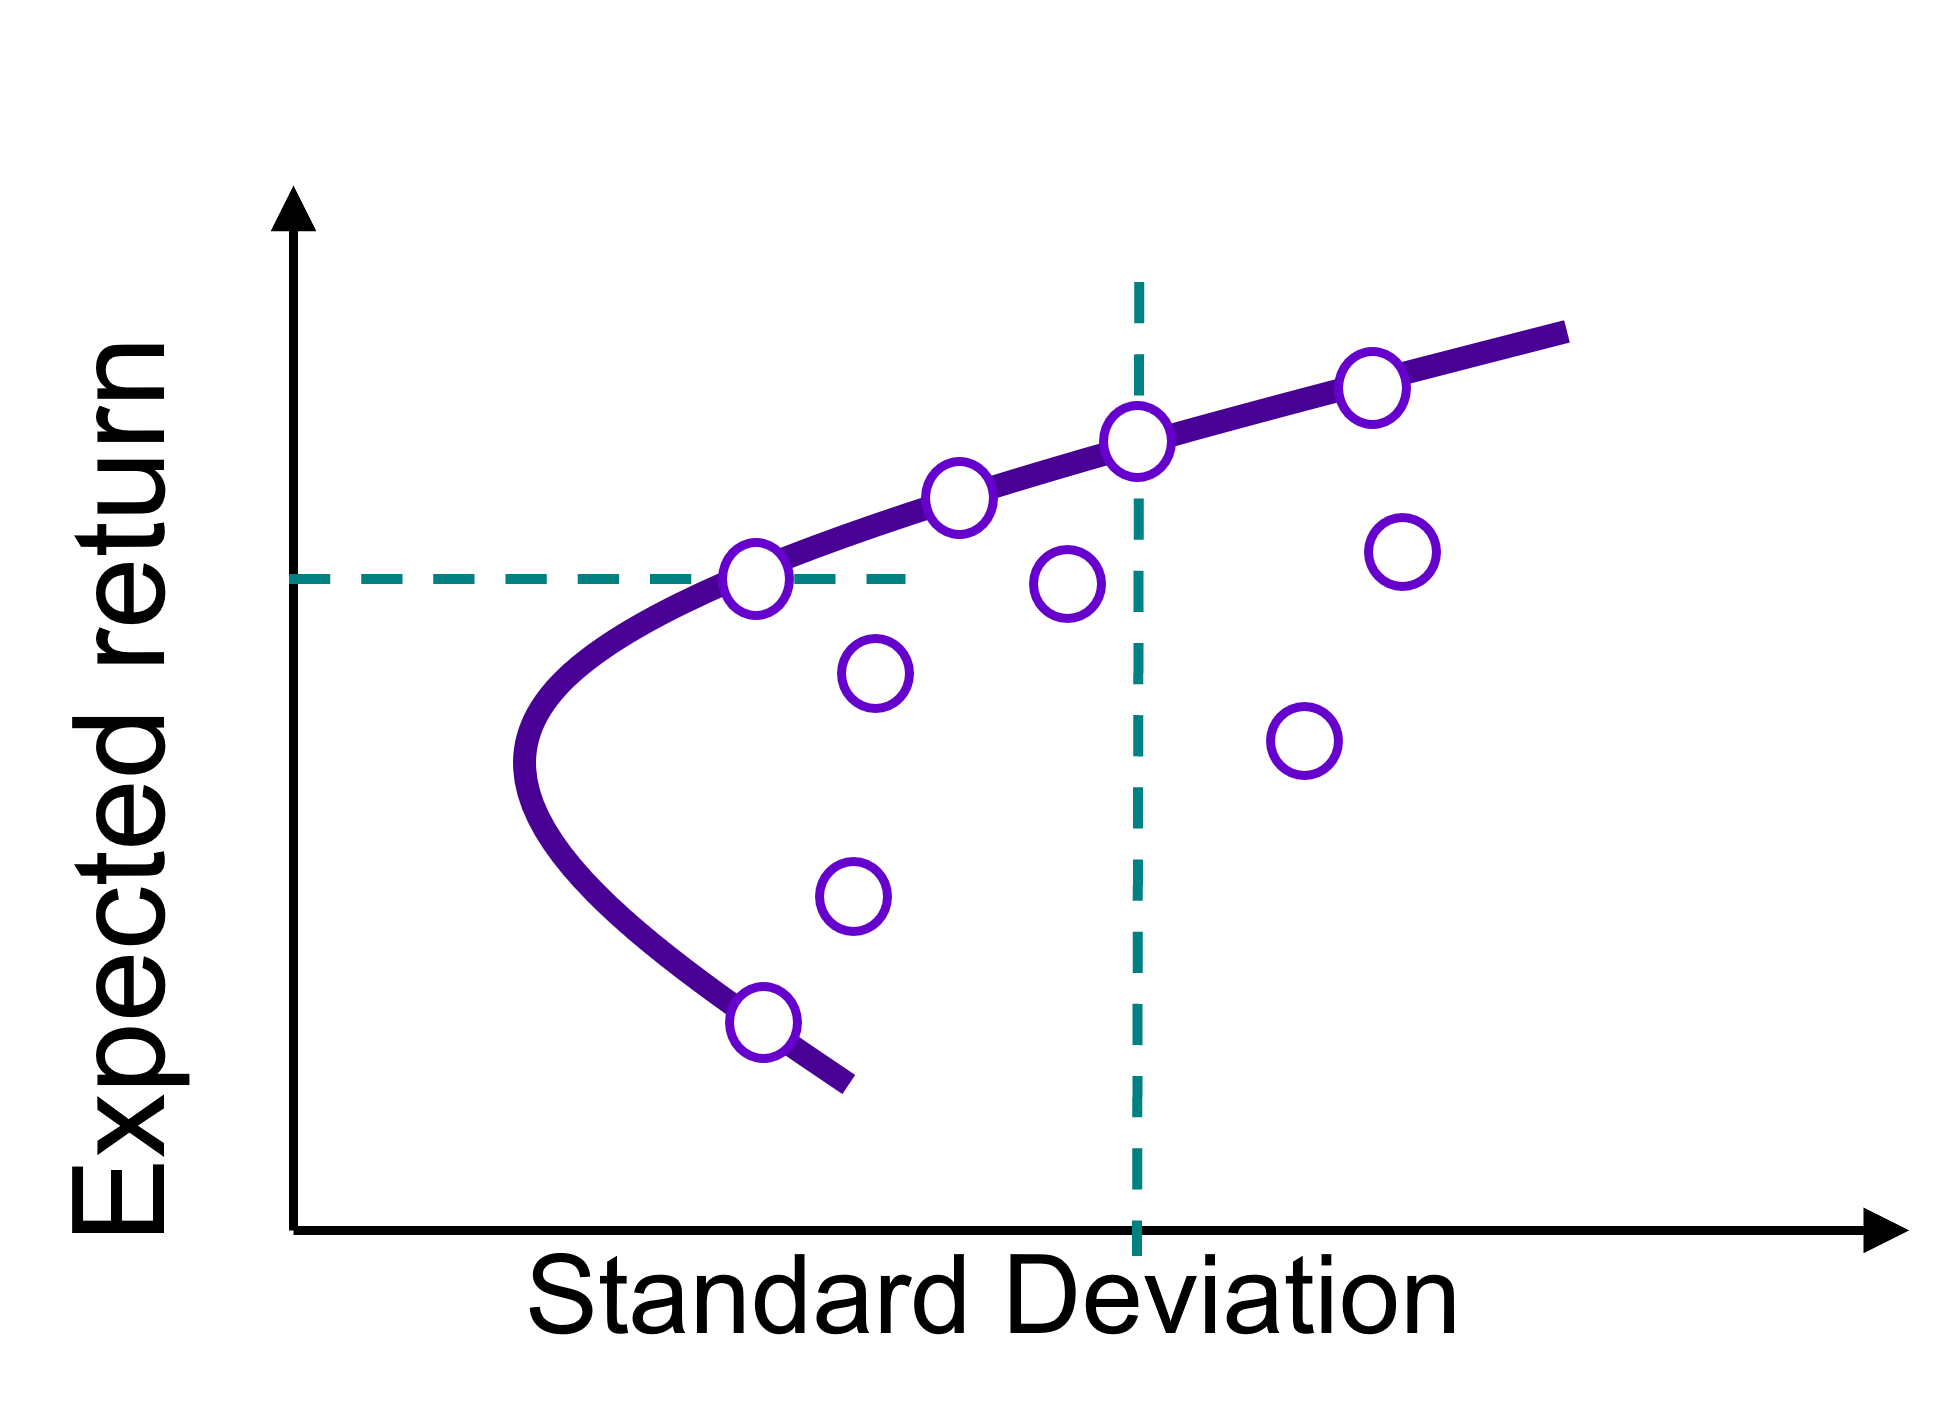
\includegraphics[width=5cm]{images/efficient_frontier.png}
\end{center}
\end{column}
\begin{column}{0.45\textwidth}
\begin{center}
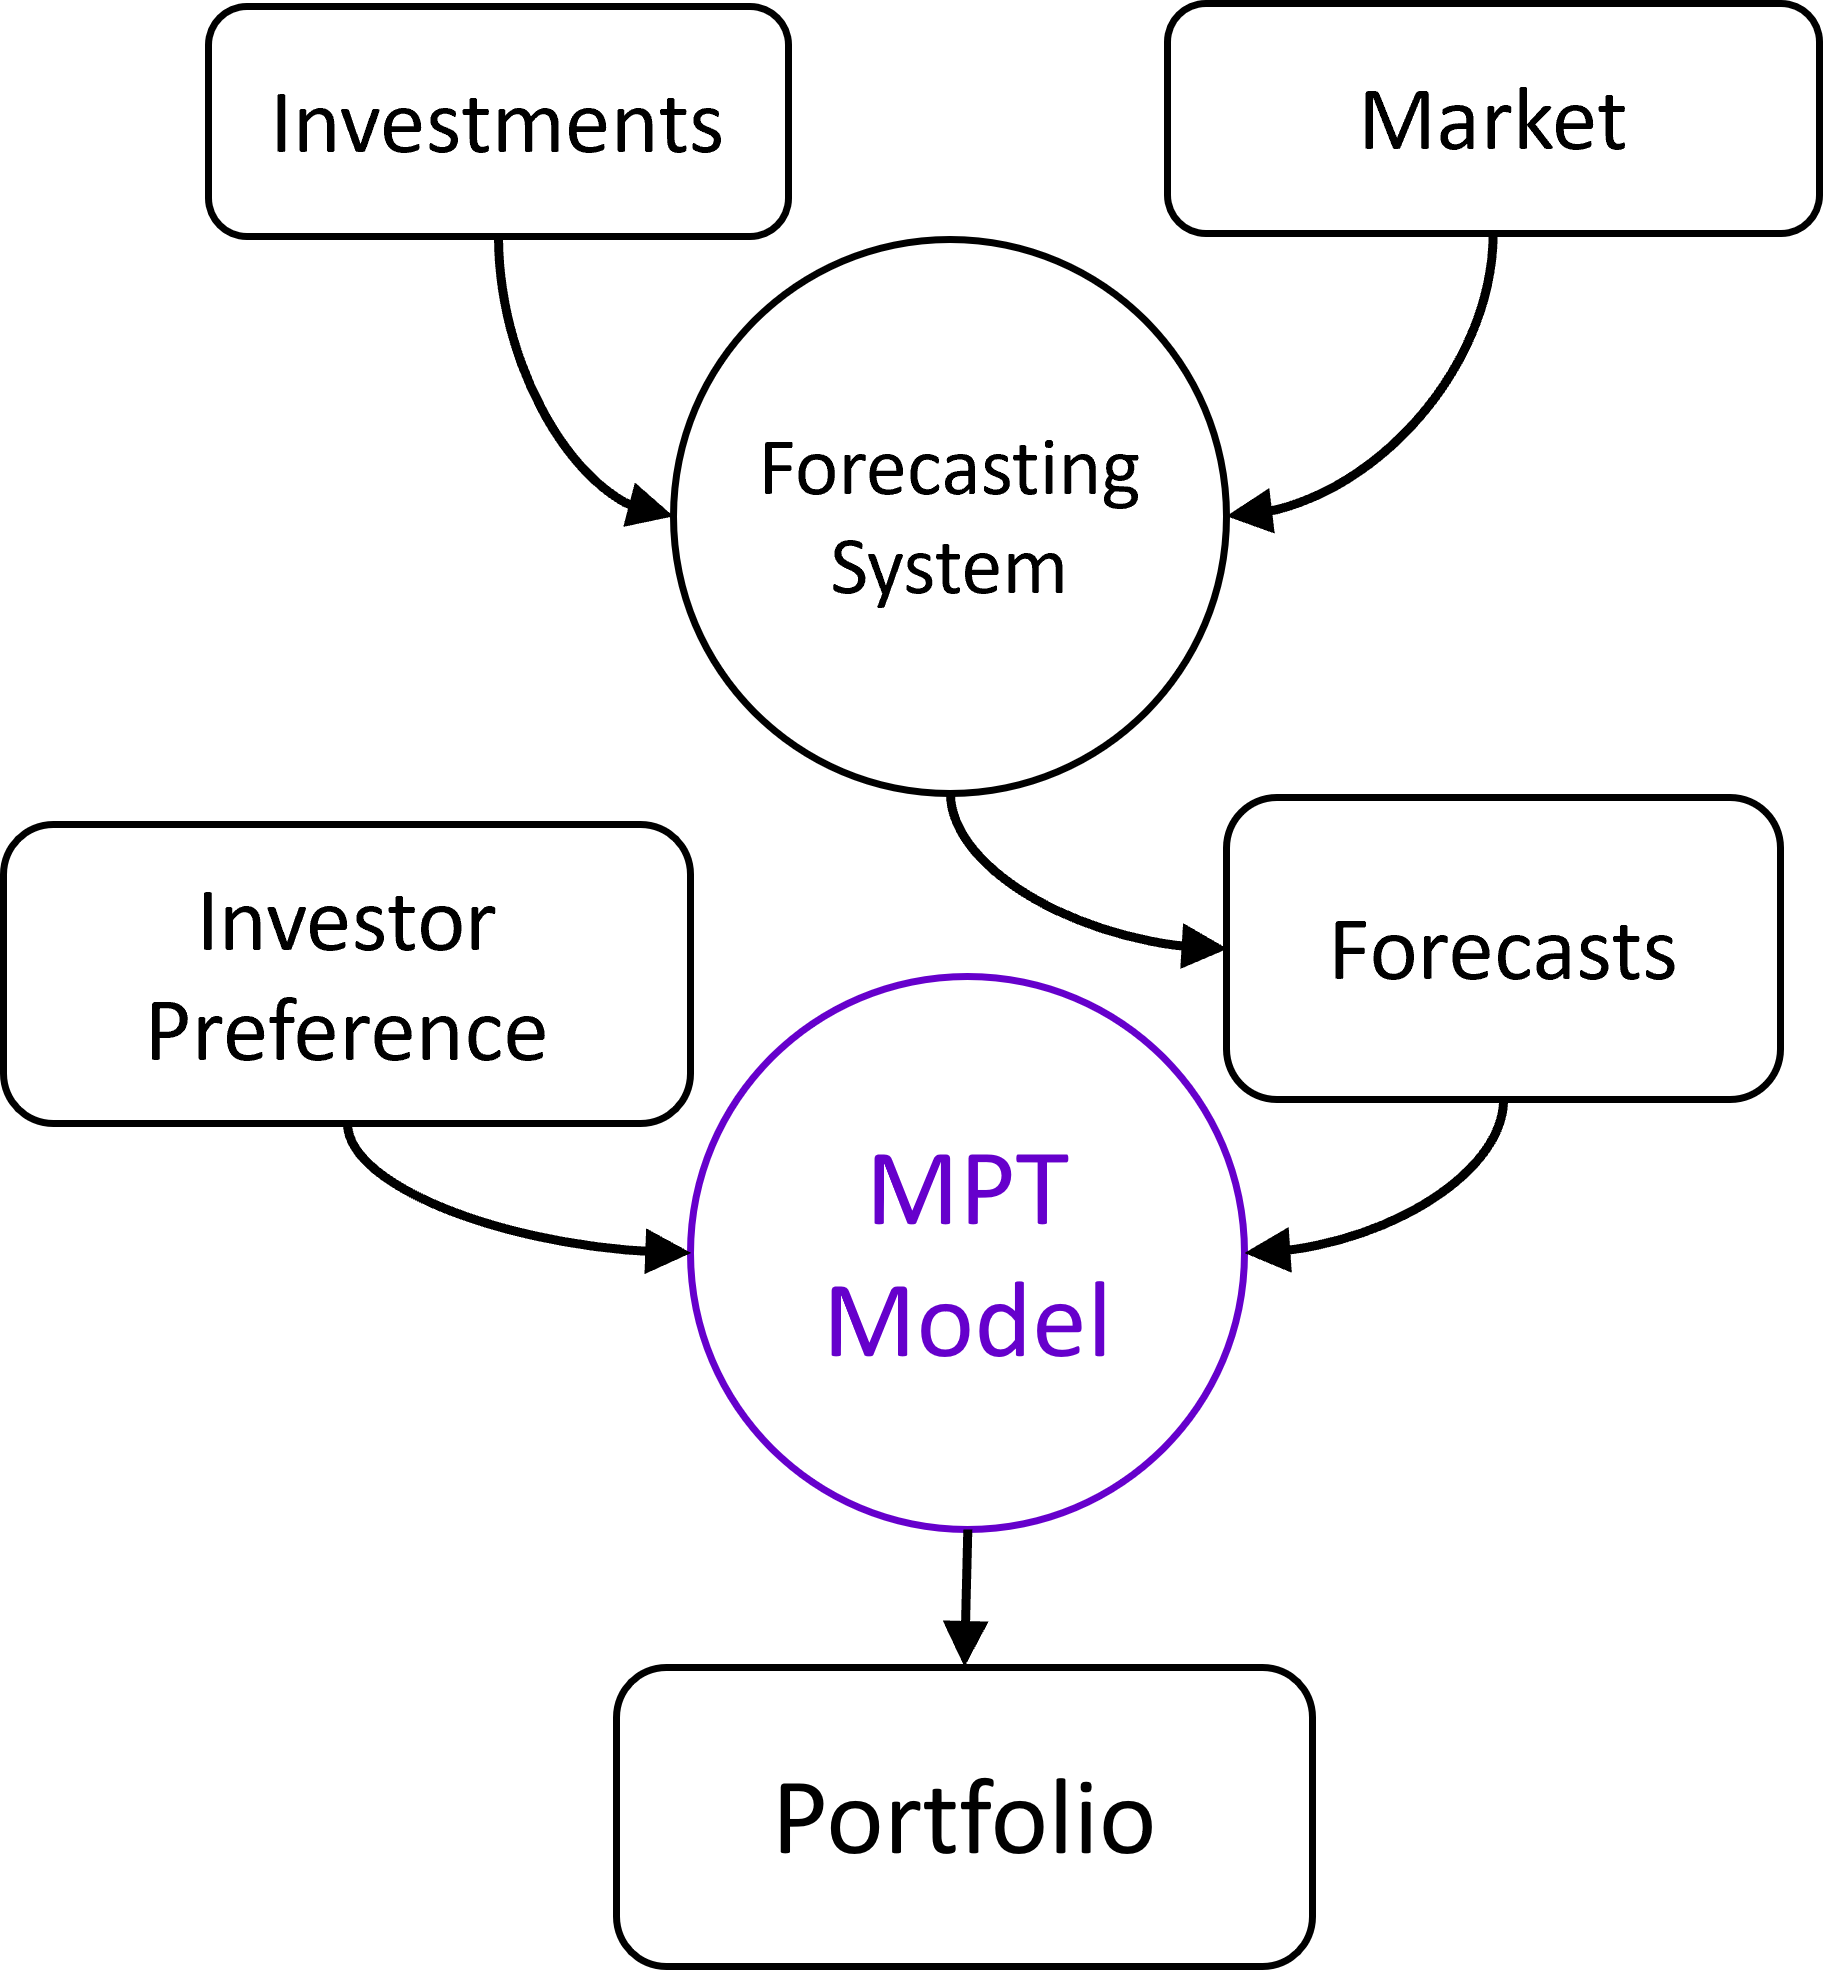
\includegraphics[width=4.8cm]{images/mpt.png}
\end{center}
\end{column}
\end{columns}
\end{frame}


\subsection{Supervised Learning Forecast System}
\begin{frame}
\frametitle{Supervised Learning Forecast System}
\begin{columns}
\begin{column}{0.55\textwidth}
\begin{itemize}
\item
Trained with labeled data.
\item The effects of transaction costs not considered.
\item
Inputs not passed to next stage, resulting in loss of information.
\end{itemize}
\end{column}
\begin{column}{0.45\textwidth}
\begin{center}
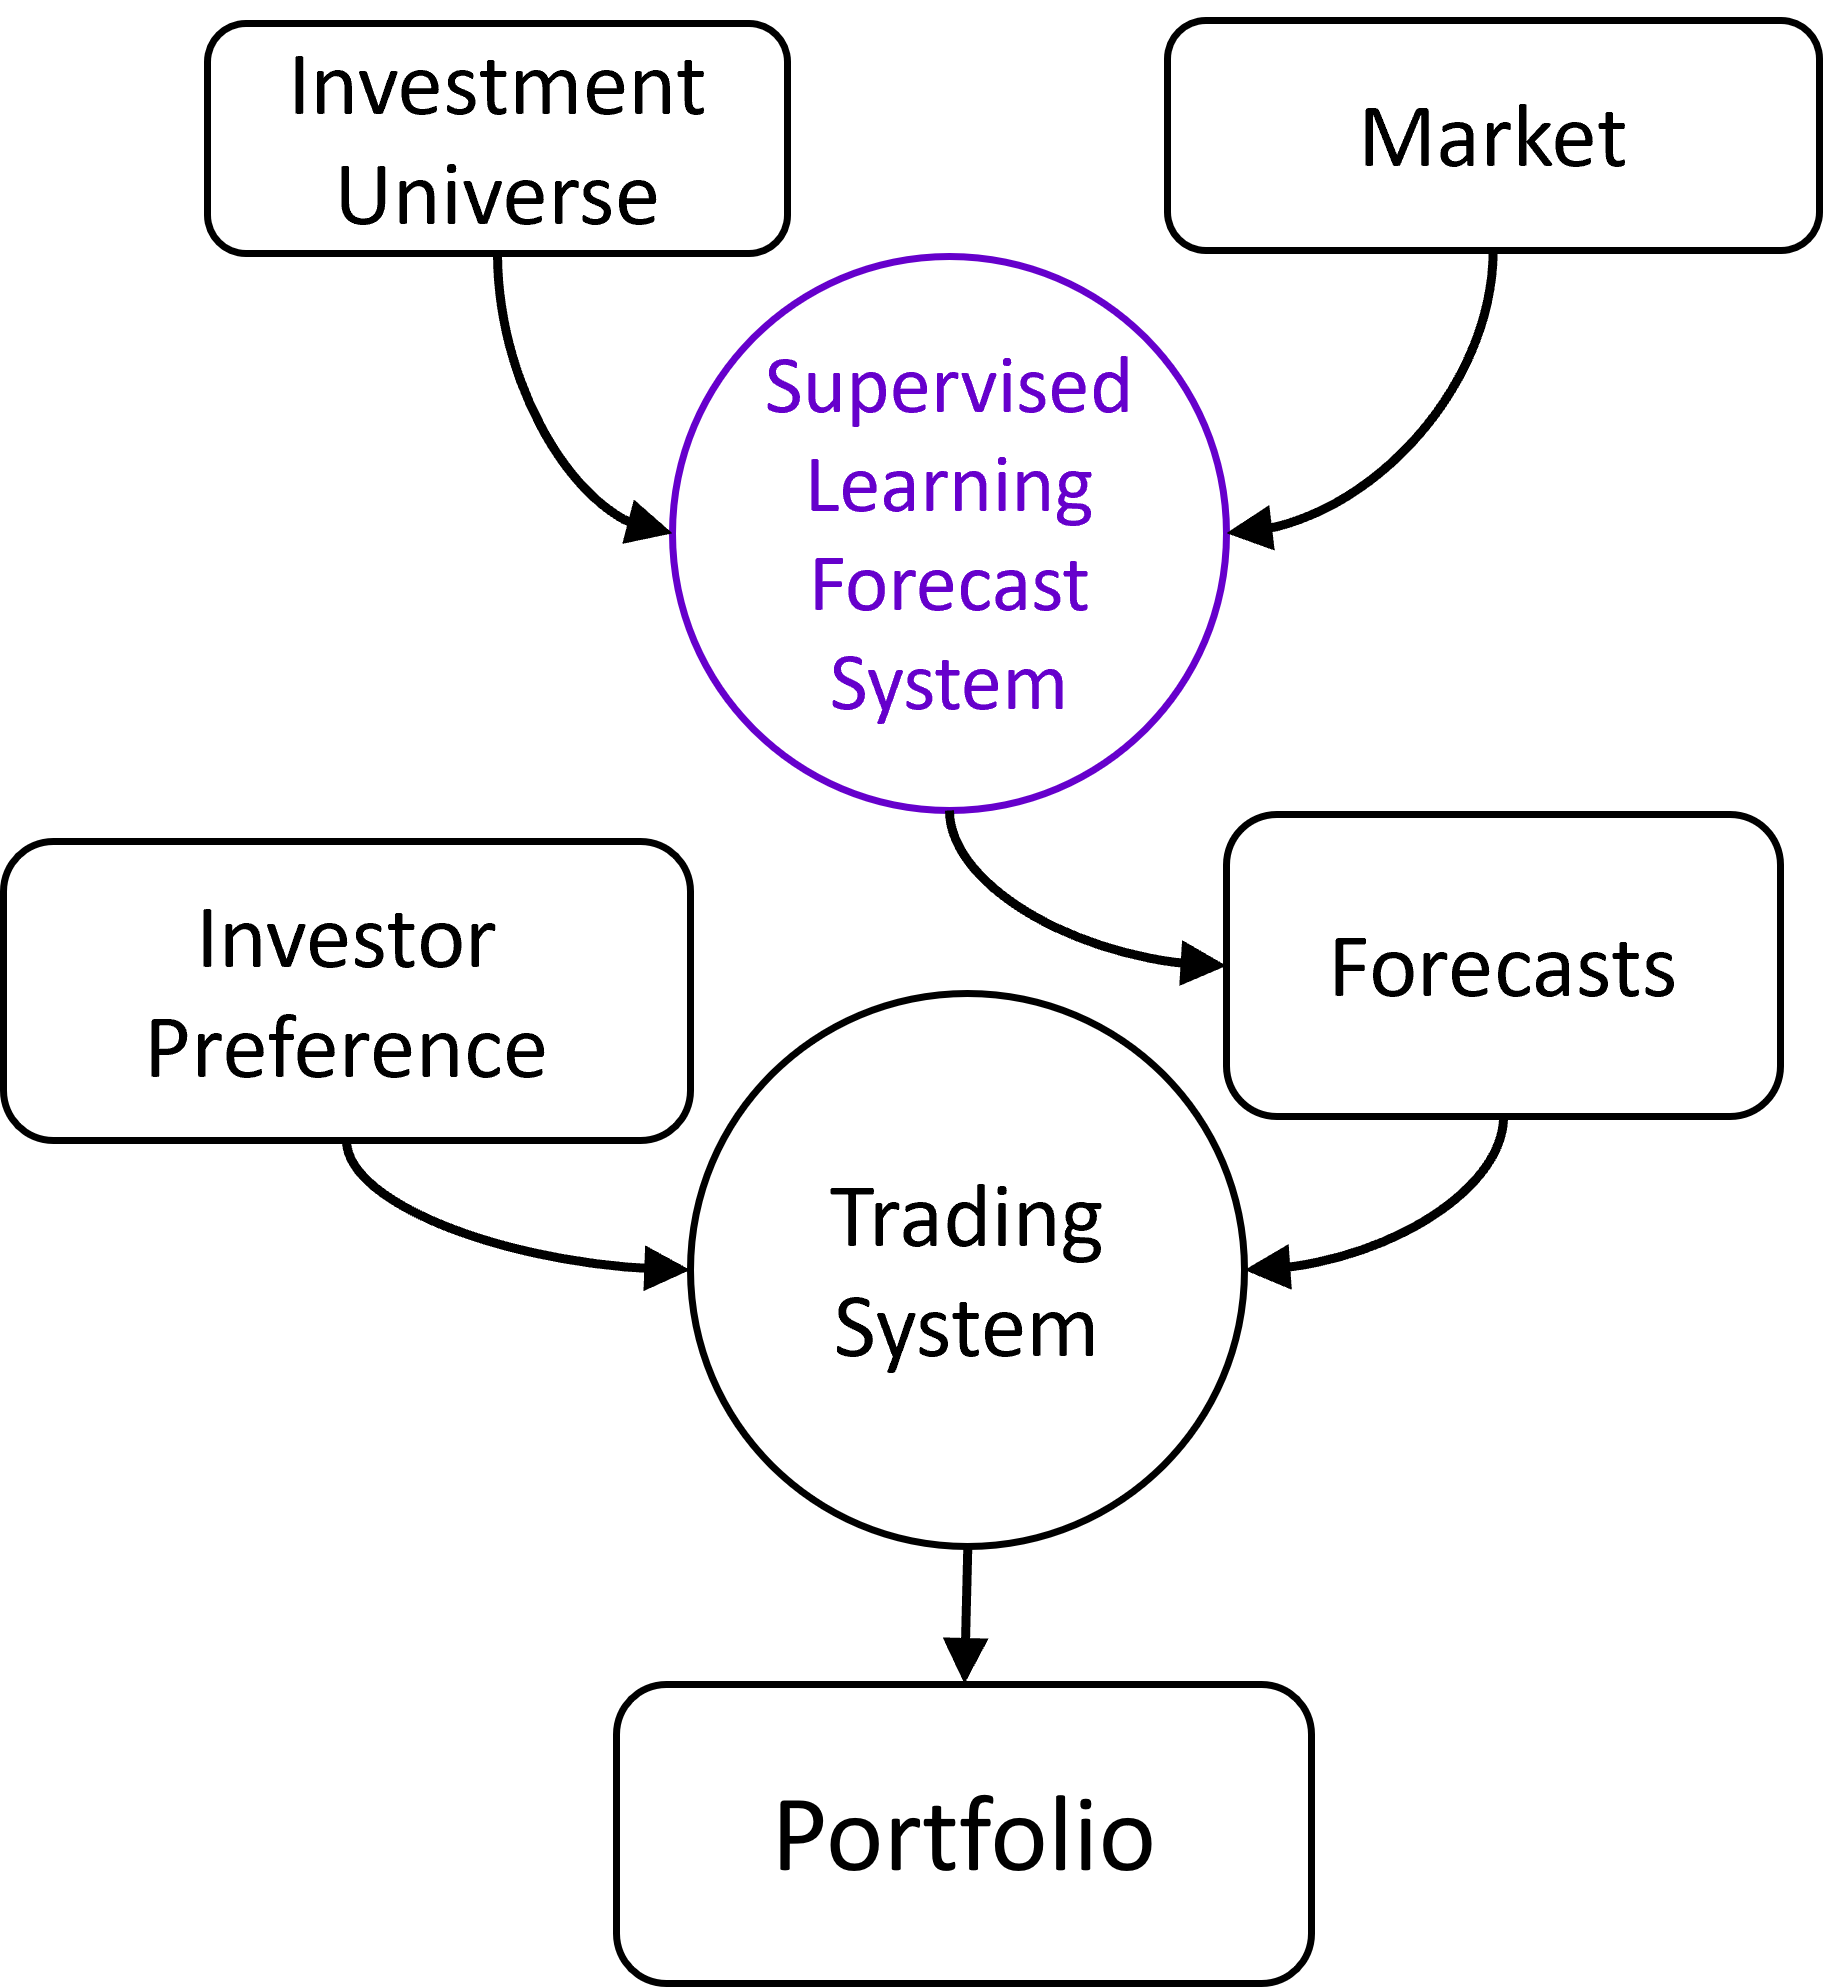
\includegraphics[width=4.8cm]{images/supervised_learning.png}
\end{center}
\end{column}
\end{columns}
\end{frame}


\subsection{Reinforcement Learning based System}
\begin{frame}
\frametitle{Reinforcement Learning (RL) based System}
\begin{columns}
\begin{column}{0.55\textwidth}
\begin{itemize}
\item
Optimize objective function directly without performance forecast.
\item
The effects of transaction costs and tax are considered.
\item
\alert
{To our knowledge, few RL-based Portfolio Management Systems incorporate with investor preference.}
\end{itemize}
\end{column}
\begin{column}{0.45\textwidth}
\begin{center}
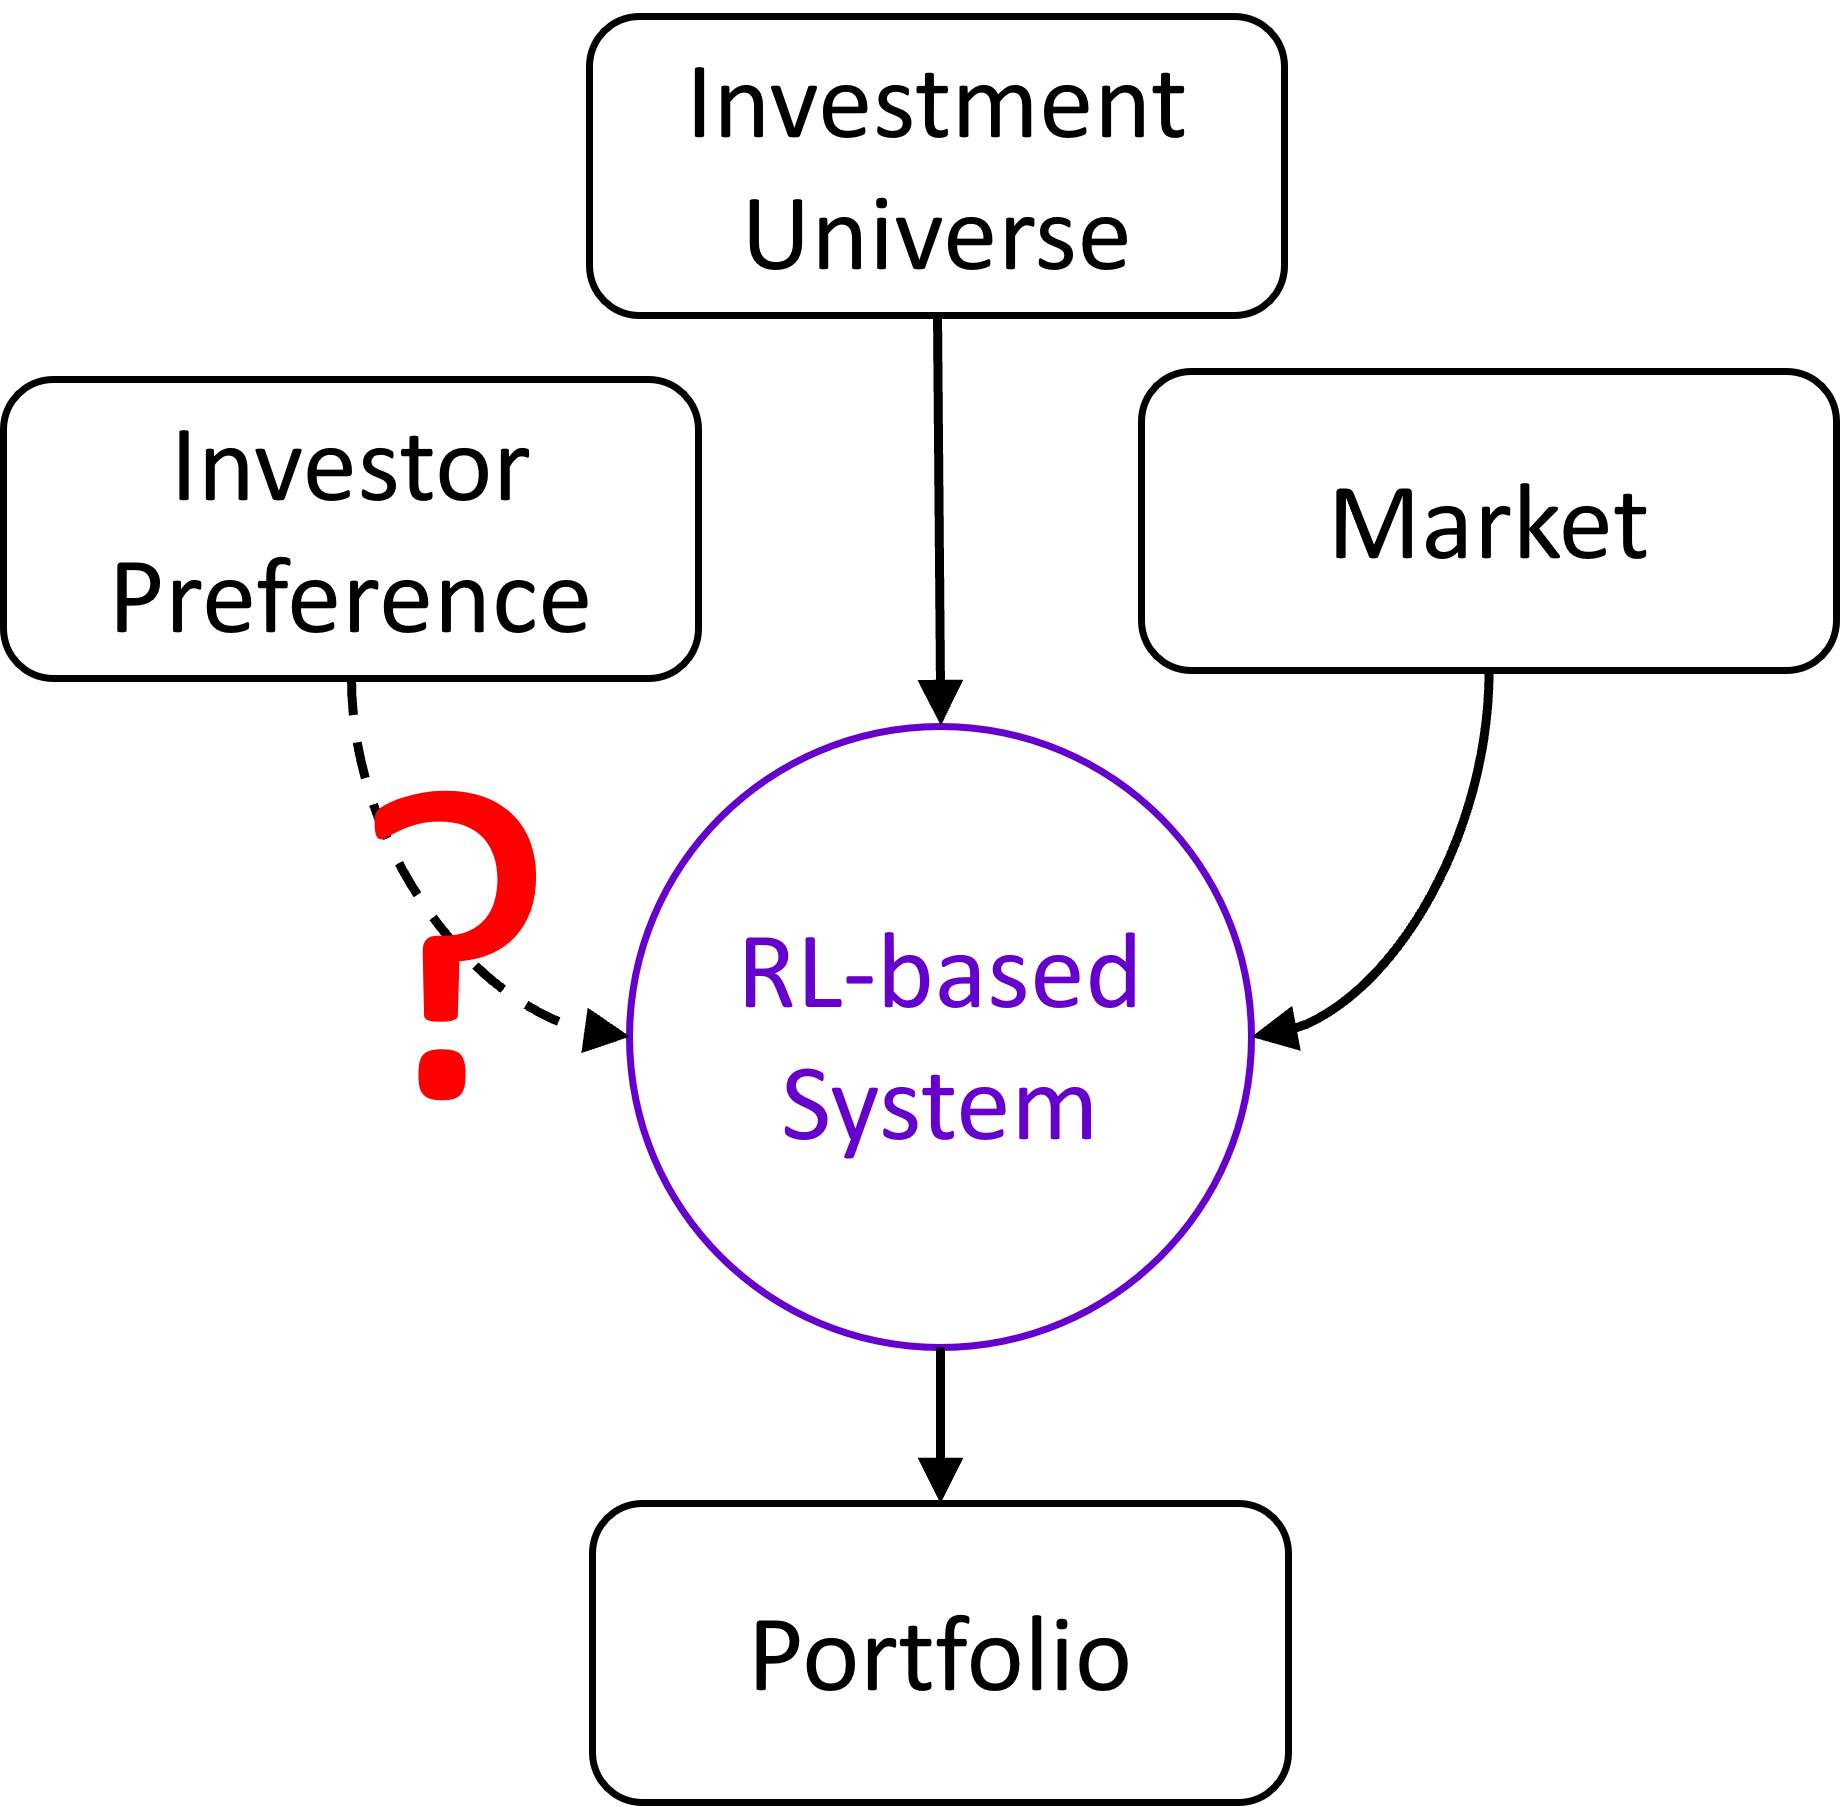
\includegraphics[width=4.8cm]{images/rl.png}
\end{center}
\end{column}
\end{columns}
\end{frame}






